
\documentclass{beamer}
\usepackage[latin1]{inputenc}
%\usetheme{Montpellier}
%\usetheme{Boadilla}
%\usecolortheme[RGB={204,51,255}]{structure}
%\usecolortheme[named=purple]{structure}
\usecolortheme[RGB={62,128,62}]{structure}
%\definecolor{reddish}{rgb}{0.3,0.15,0.3}
%\definecolor{light}{rgb}{0.8,0.6,0.8}
%\definecolor{reddish}{rgb}{.5,0.15,0.15}
\definecolor{reddish}{rgb}{0.5,0.3,0.4}
%\definecolor{light}{rgb}{0.8,0.6,0.8}
\definecolor{reddish}{rgb}{.7,0.25,0.25}
\definecolor{greenish}{rgb}{.25,0.8,0.25}
\definecolor{blueish}{rgb}{.25,0.25,0.7}
\definecolor{purple}{rgb}{.5,0.0,0.5}
\usepackage{graphicx}
\usepackage{pstricks}

\newcommand{\btVFill}{\vskip0pt plus 1filll}

\setbeamertemplate{navigation symbols}{}

\newcommand{\crish}{\color{reddish}}
\newcommand{\cgish}{\color{greenish}}
\newcommand{\cbla}{\color{black}}
\newcommand{\cred}{\color{red}}
\newcommand{\cblu}{\color{blue}}
\newcommand{\cgrish}{\color{green}}

\newcommand{\sm}{\color{reddish}$}
\newcommand{\fm}{$\color{black}{}}

\newcommand{\letter}[1]{\color{blue}\texttt{#1}\color{black}}
\newcommand{\binary}[1]{\color{red}\texttt{#1}\color{black}}

\usepackage{tikz}
\usetikzlibrary{arrows,decorations.markings,positioning}
\usepackage{epstopdf}
\usetikzlibrary{fit}
\usepackage{pgfplots}

\title[Information Theory lecture 10]{The cocktail party problem: information theory lecture 10}
\author{COMSM0075 Information Processing and Brain}
\institute{\texttt{comsm0075.github.io}}
\date{October 2020}

\begin{document}

\maketitle

\begin{frame}{The cocktail party problem}
  \begin{center}
    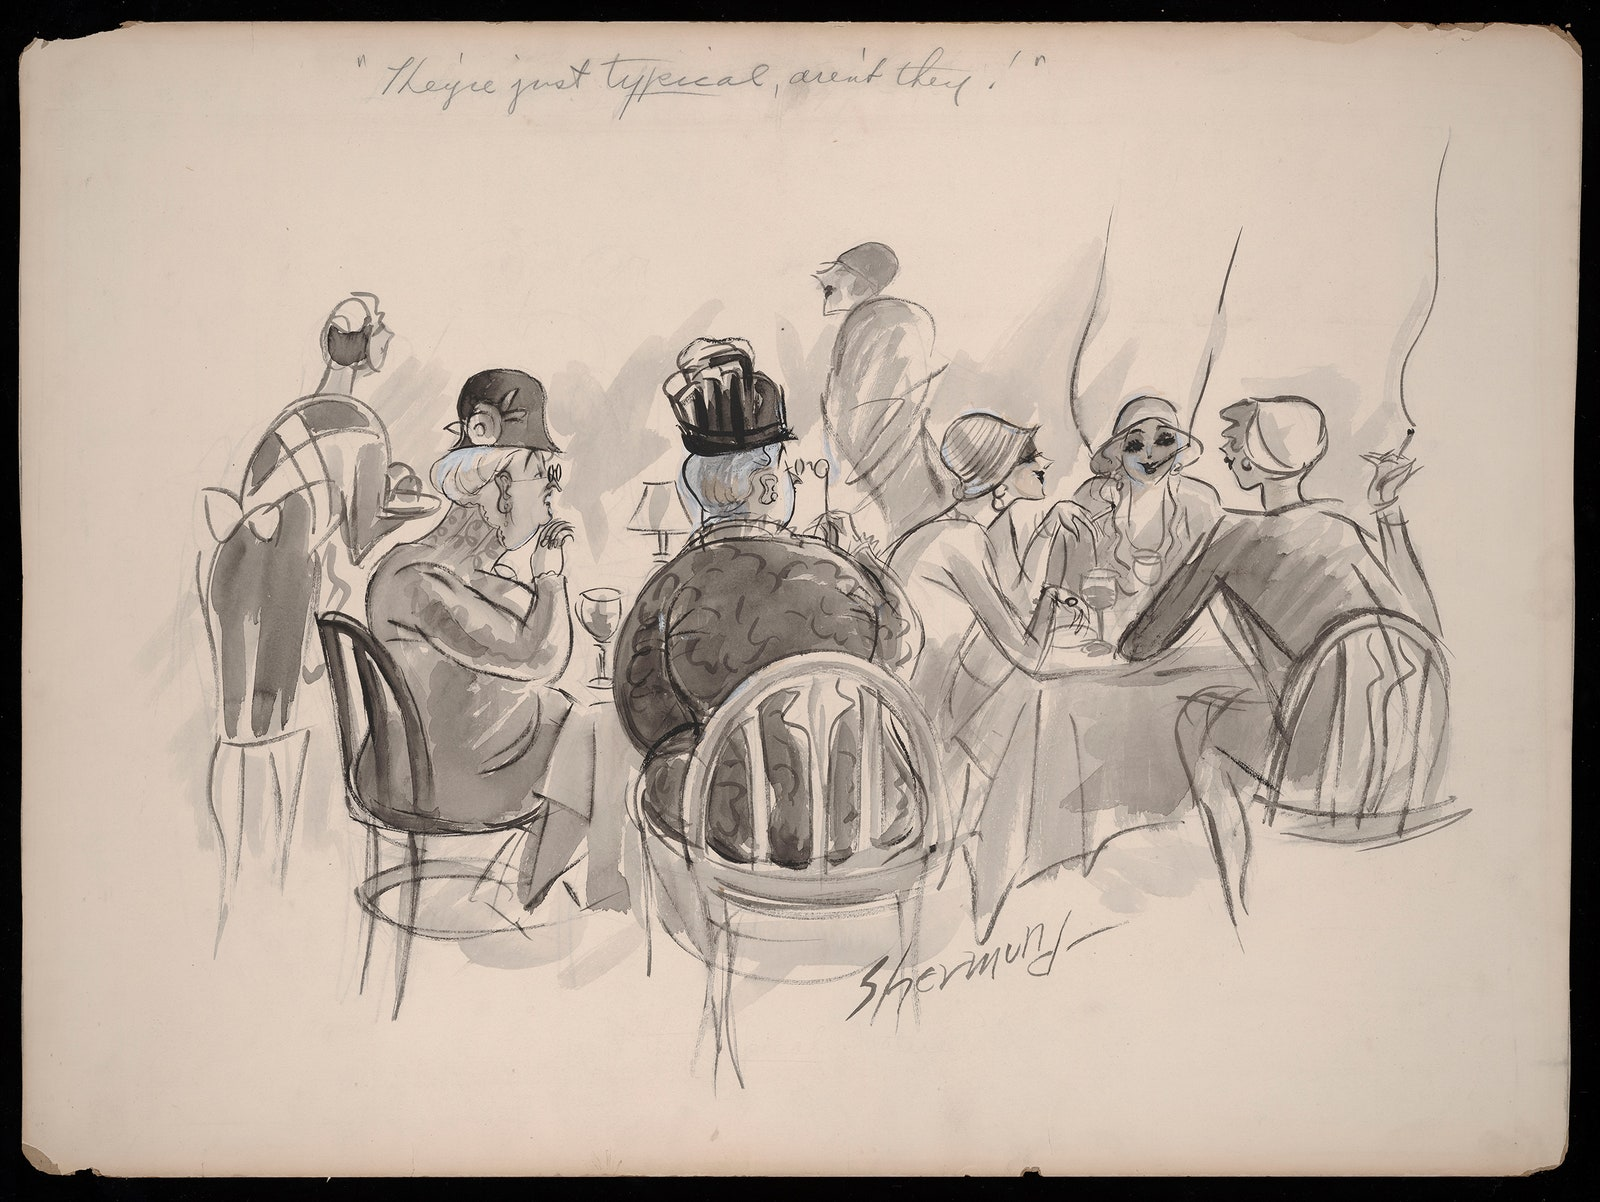
\includegraphics[width=10cm]{Barbara_Shermund.jpg}
  \end{center}
   \vfill
\flushright{\tiny{\cred{}Cartoon by Barbara Shermund.\cbla{}}}
\end{frame}


\begin{frame}{The cocktail party problem}
  \begin{center}
    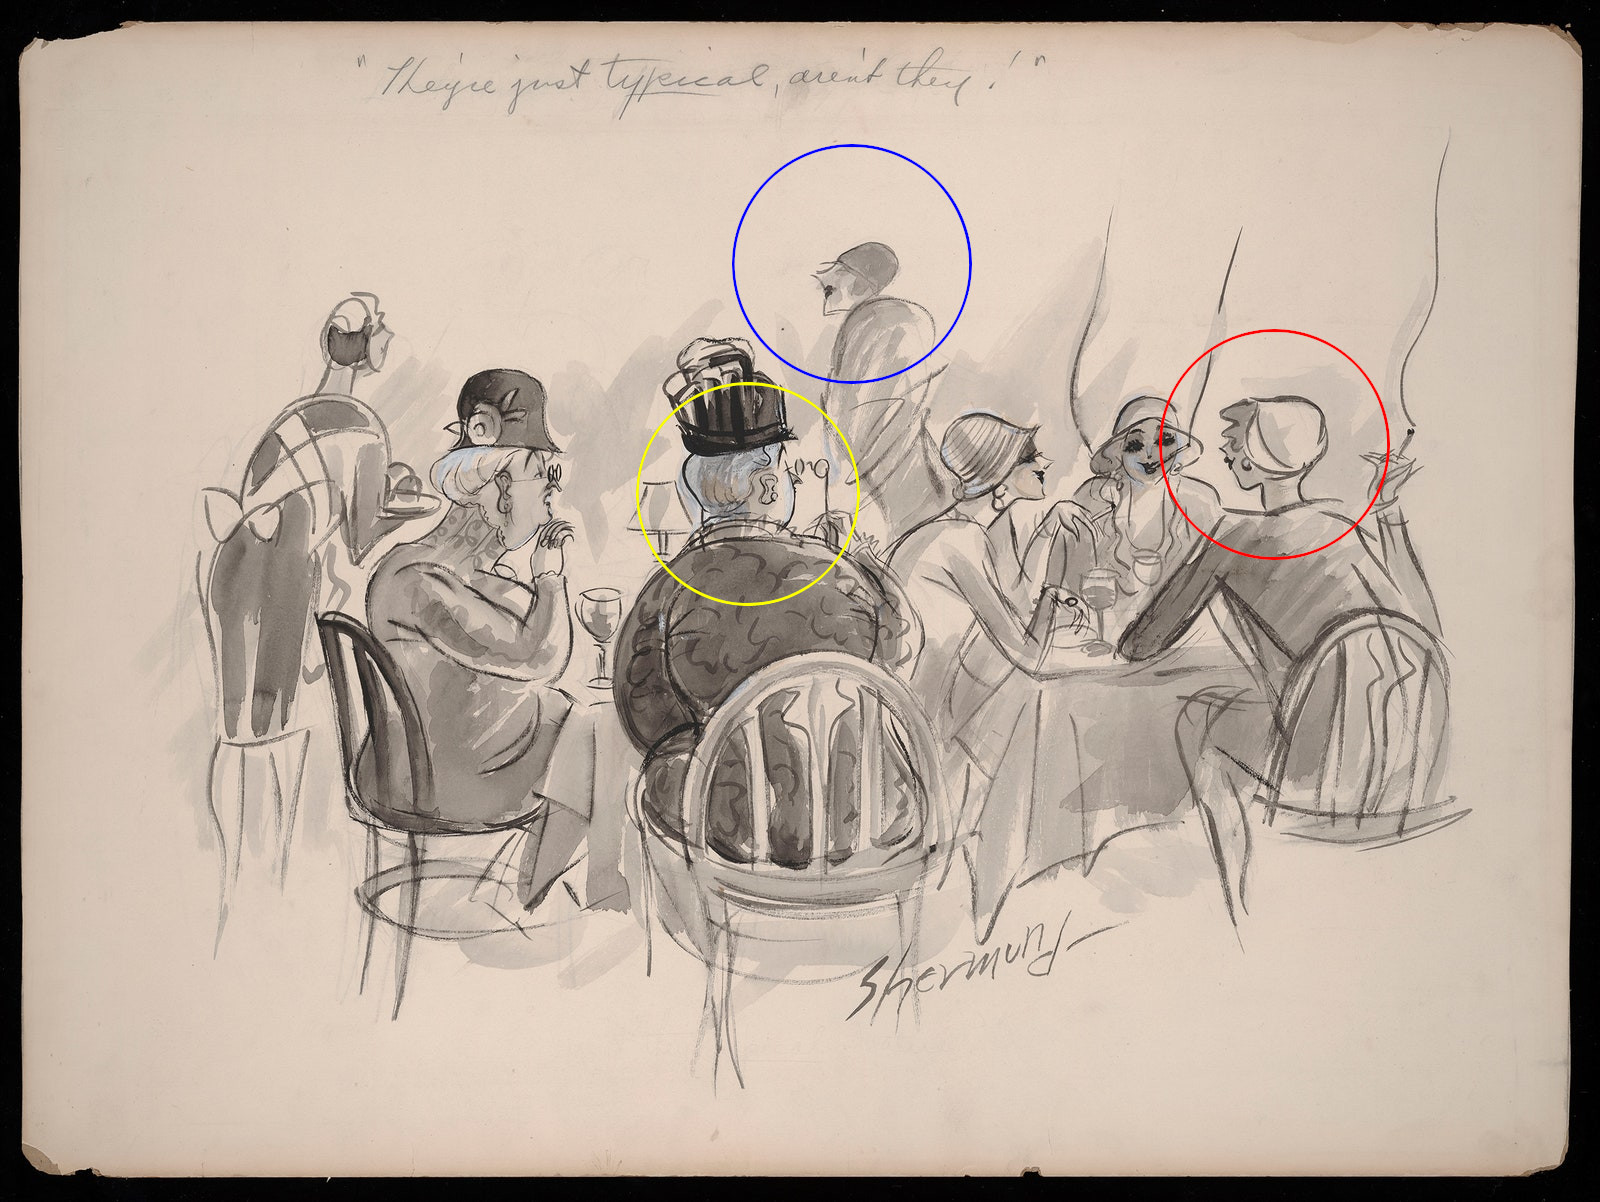
\includegraphics[width=10cm]{Barbara_Shermund_circles.jpg}
  \end{center}
   \vfill
\flushright{\tiny{\cred{}Cartoon by Barbara Shermund.\cbla{}}}
\end{frame}


\begin{frame}{The cocktail party problem}
  \begin{center}
    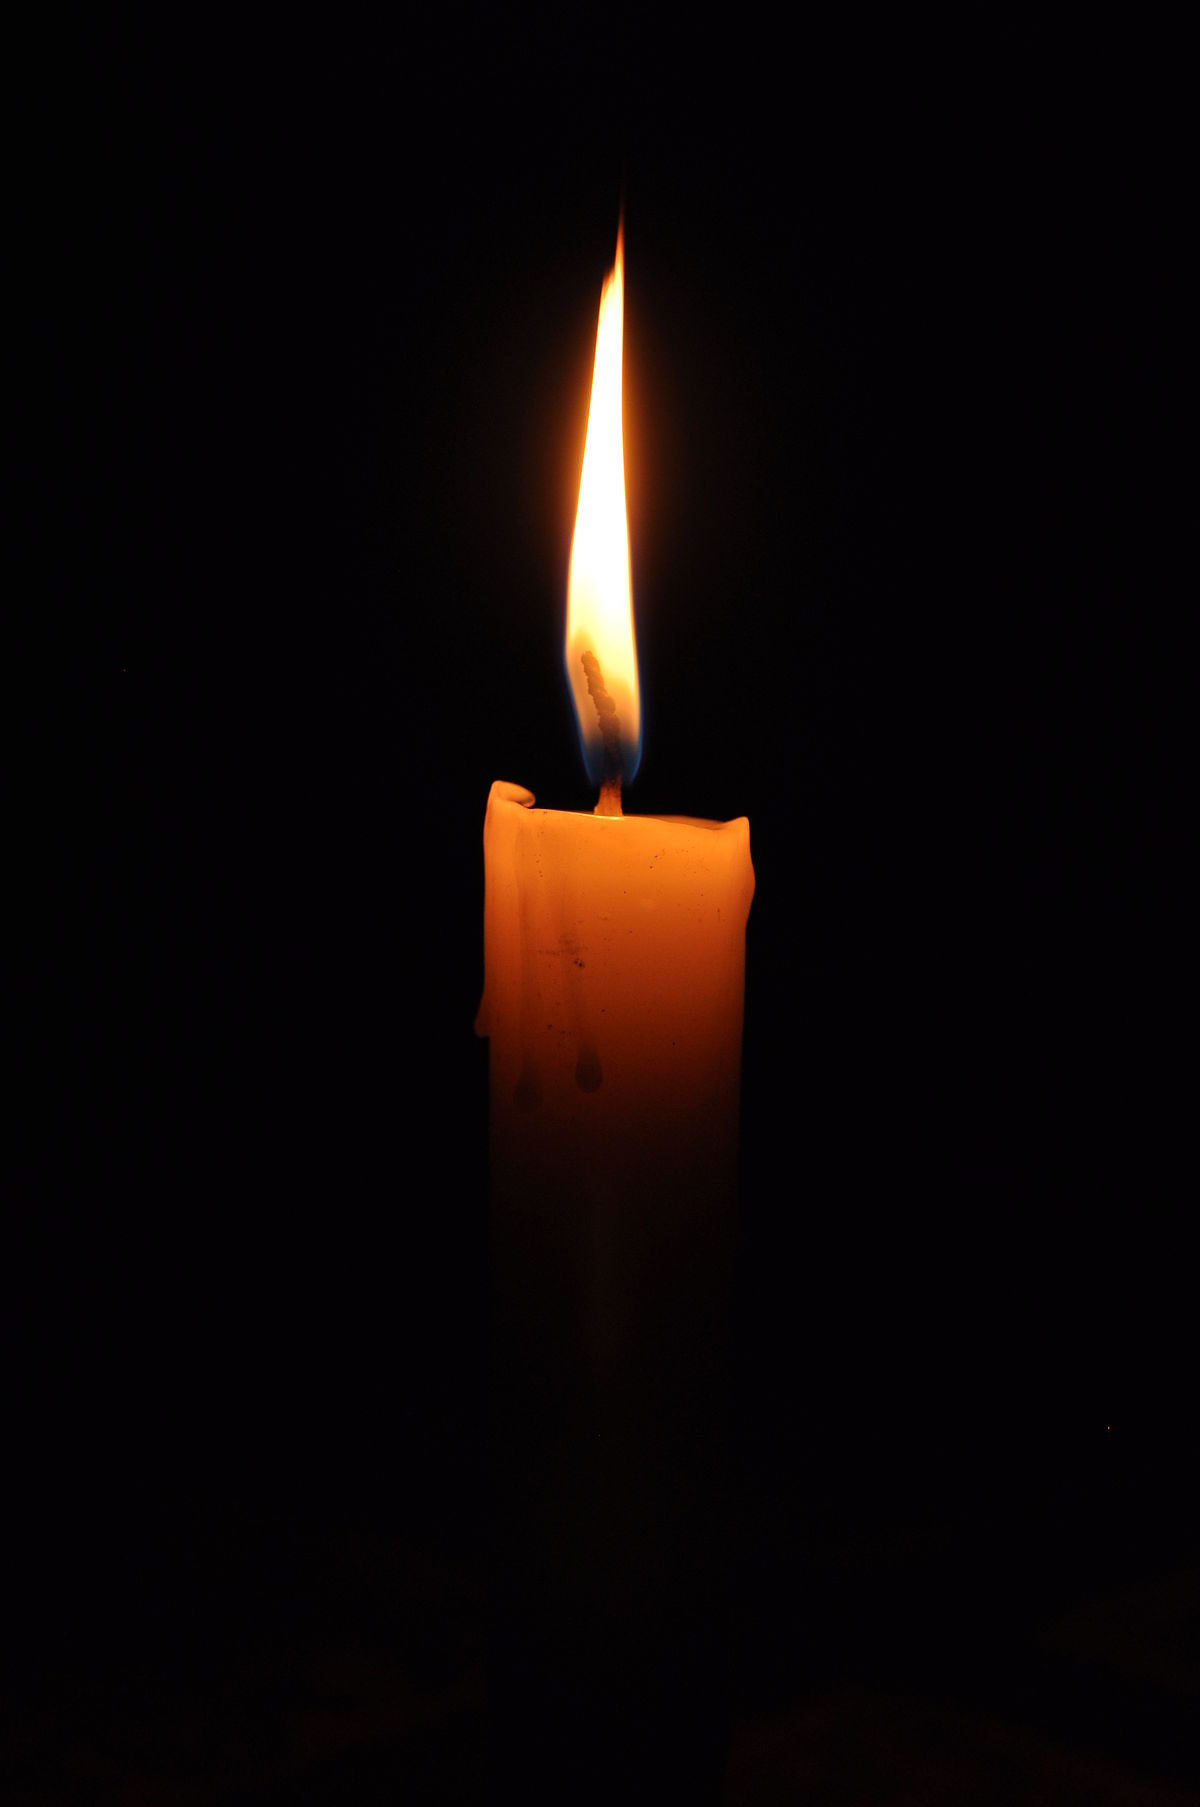
\includegraphics[width=3cm]{Candle.jpg}
  \end{center}
   \vfill
\flushright{\tiny{\cred{}Image from wikipedia.\cbla{}}}
\end{frame}


\begin{frame}{The cocktail party problem}
  \begin{center}
    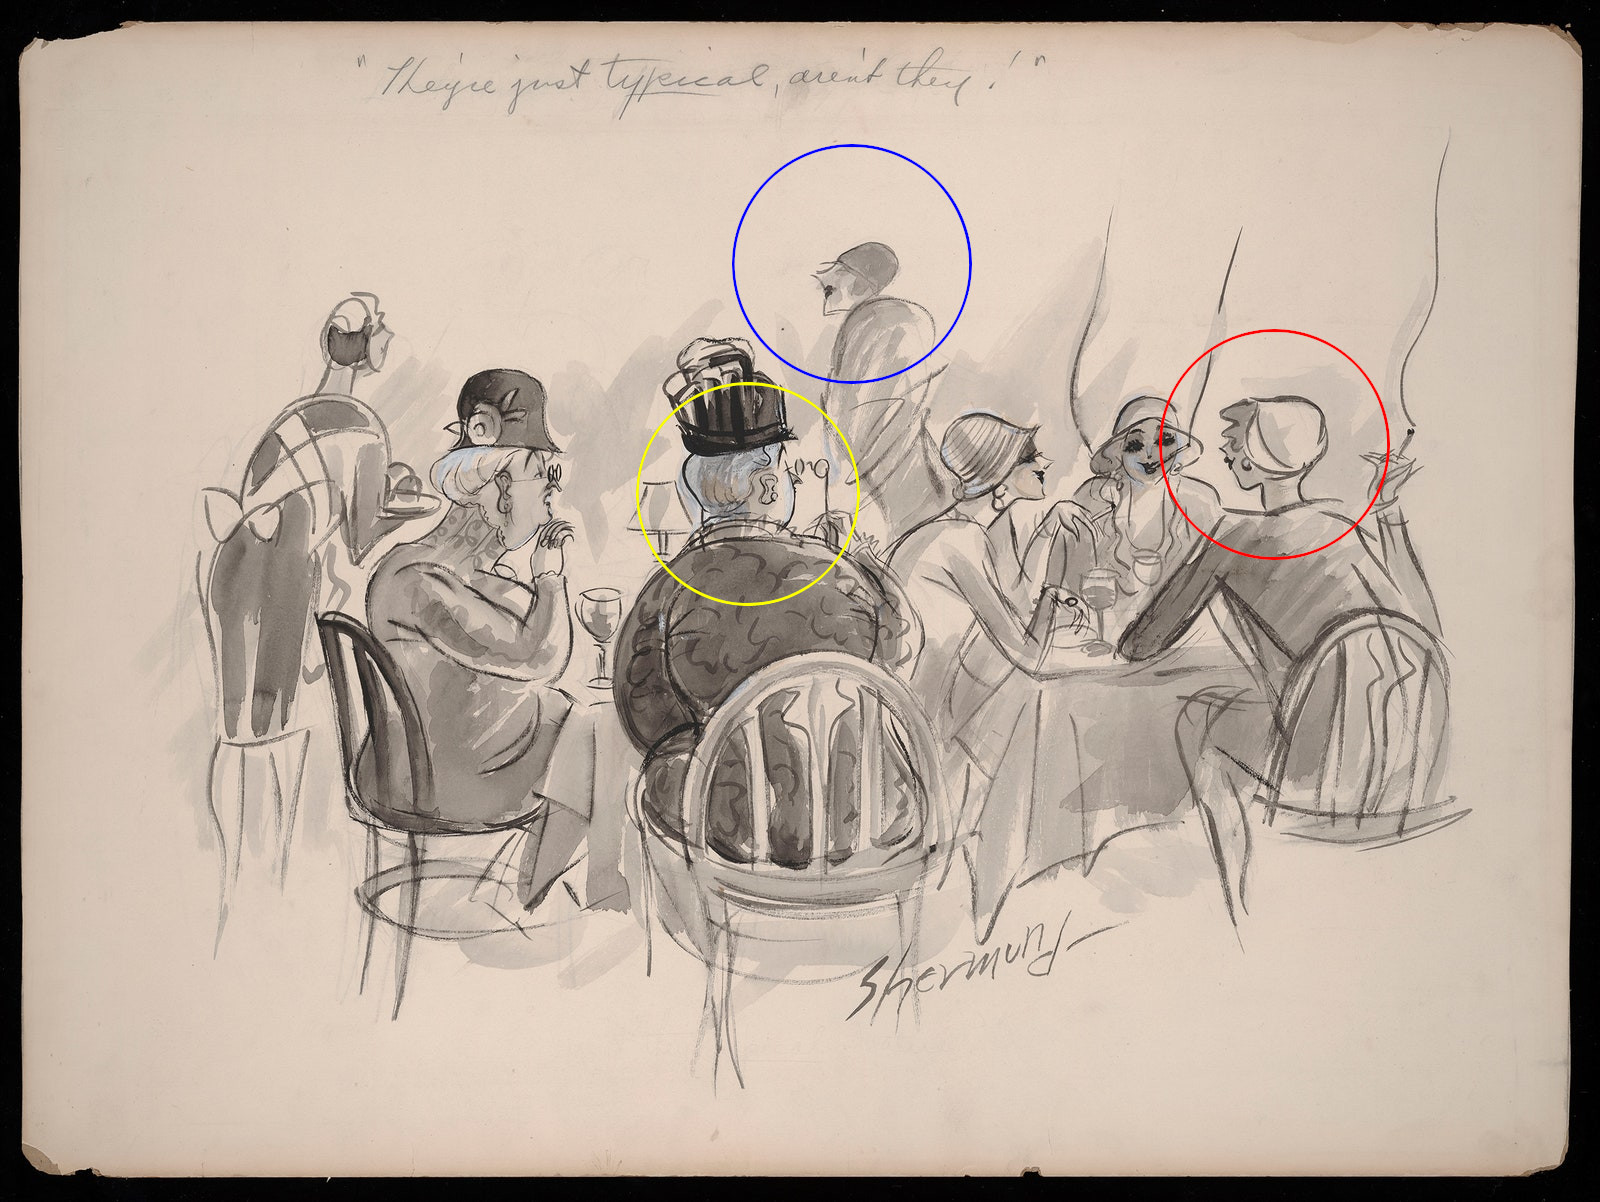
\includegraphics[width=10cm]{Barbara_Shermund_circles.jpg}
  \end{center}
   \vfill
\flushright{\tiny{\cred{}Cartoon by Barbara Shermund.\cbla{}}}
\end{frame}


\begin{frame}{The cocktail party problem}
  \begin{center}
    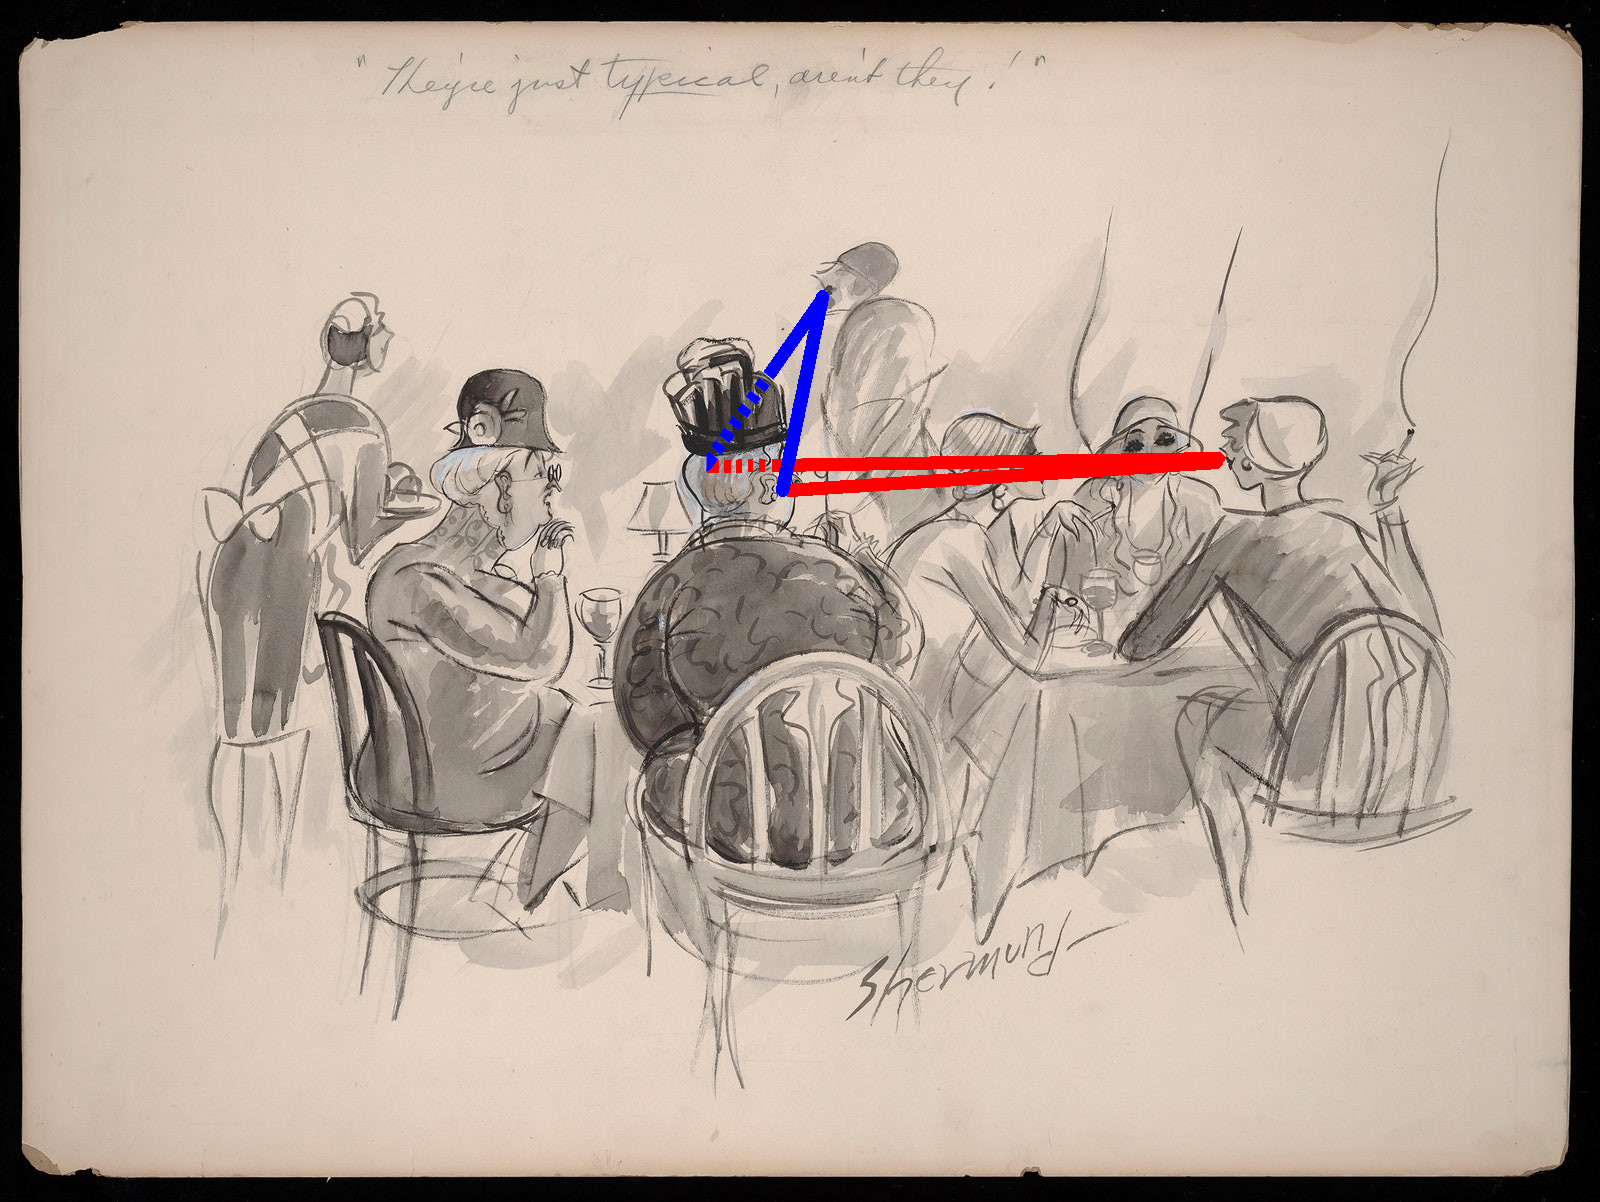
\includegraphics[width=10cm]{Barbara_Shermund_lines.jpg}
  \end{center}
   \vfill
\flushright{\tiny{\cred{}Cartoon by Barbara Shermund.\cbla{}}}
\end{frame}

\begin{frame}{The cocktail party problem}
  \begin{center}
    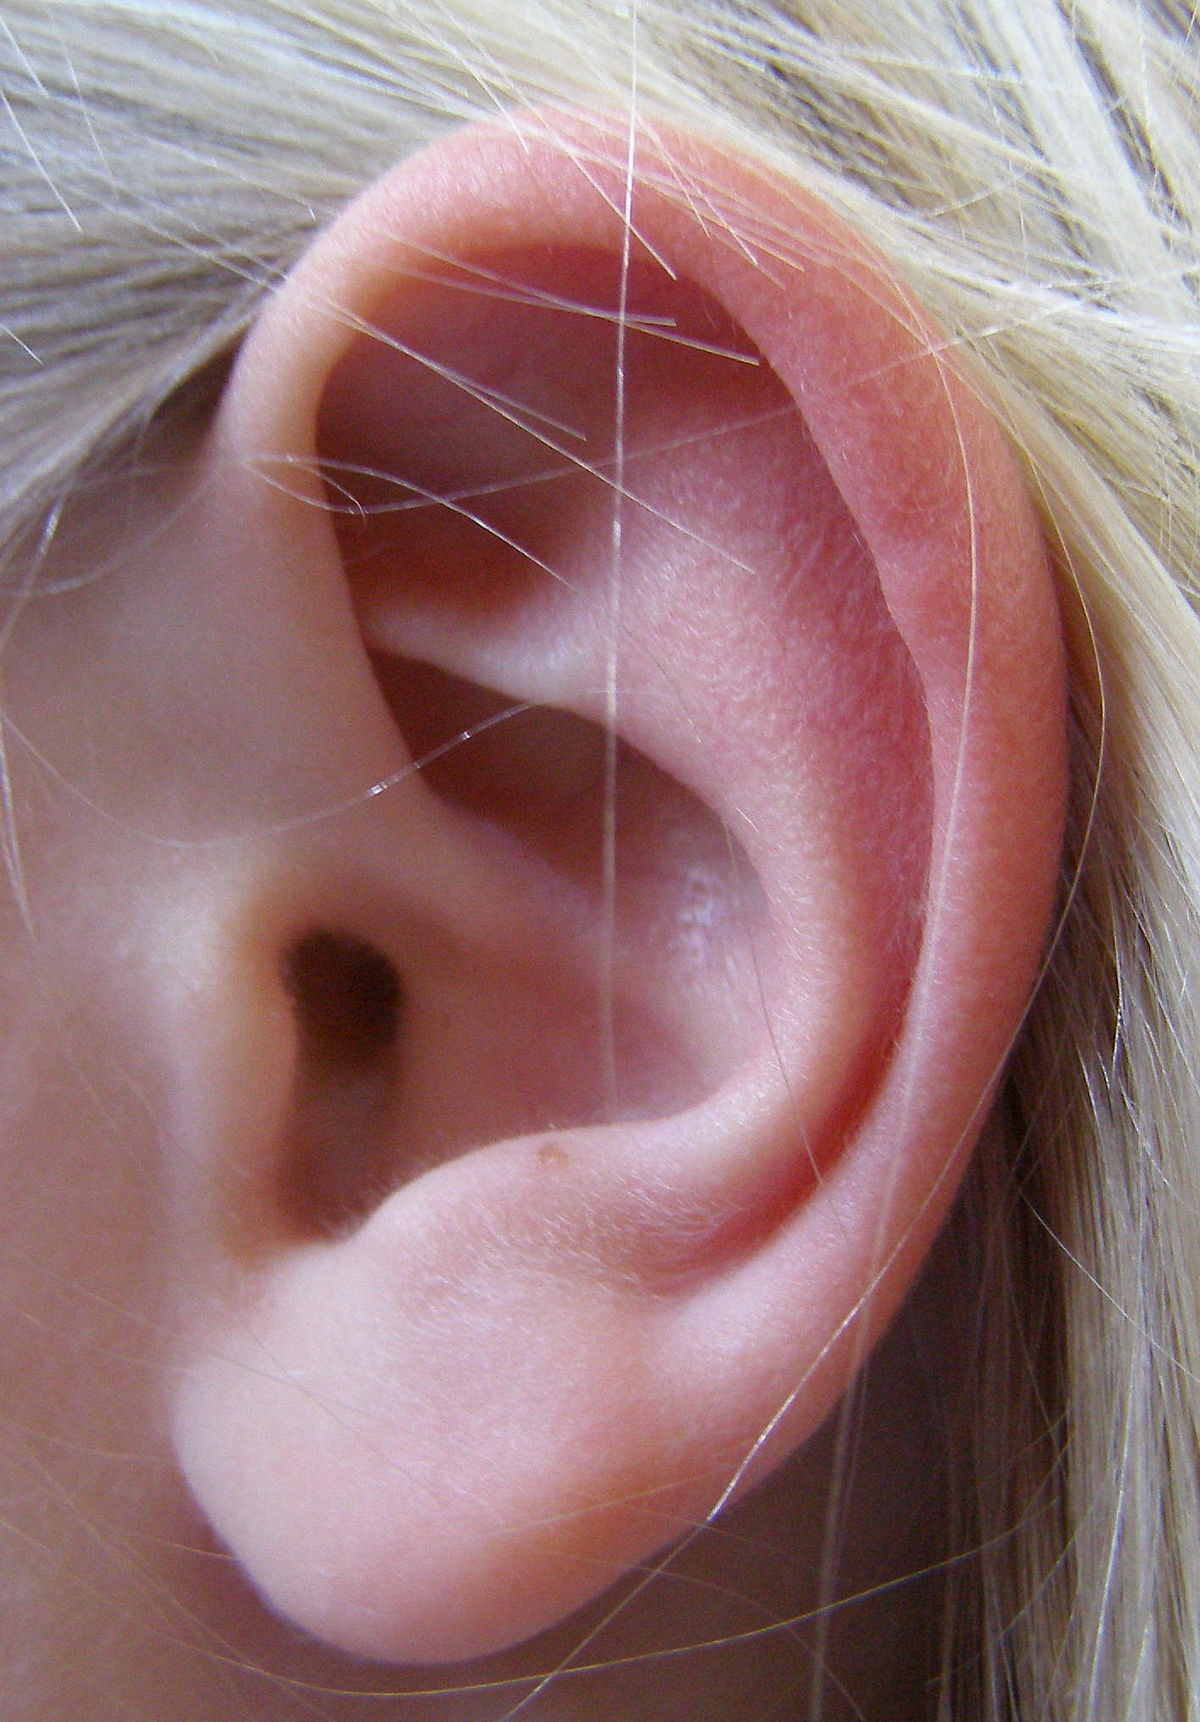
\includegraphics[width=3cm]{ear.jpg}
  \end{center}
   \vfill
\flushright{\tiny{\cred{}Image from wikipedia.\cbla{}}}
\end{frame}


\begin{frame}{The cocktail party problem - simple version}
  \begin{center}
    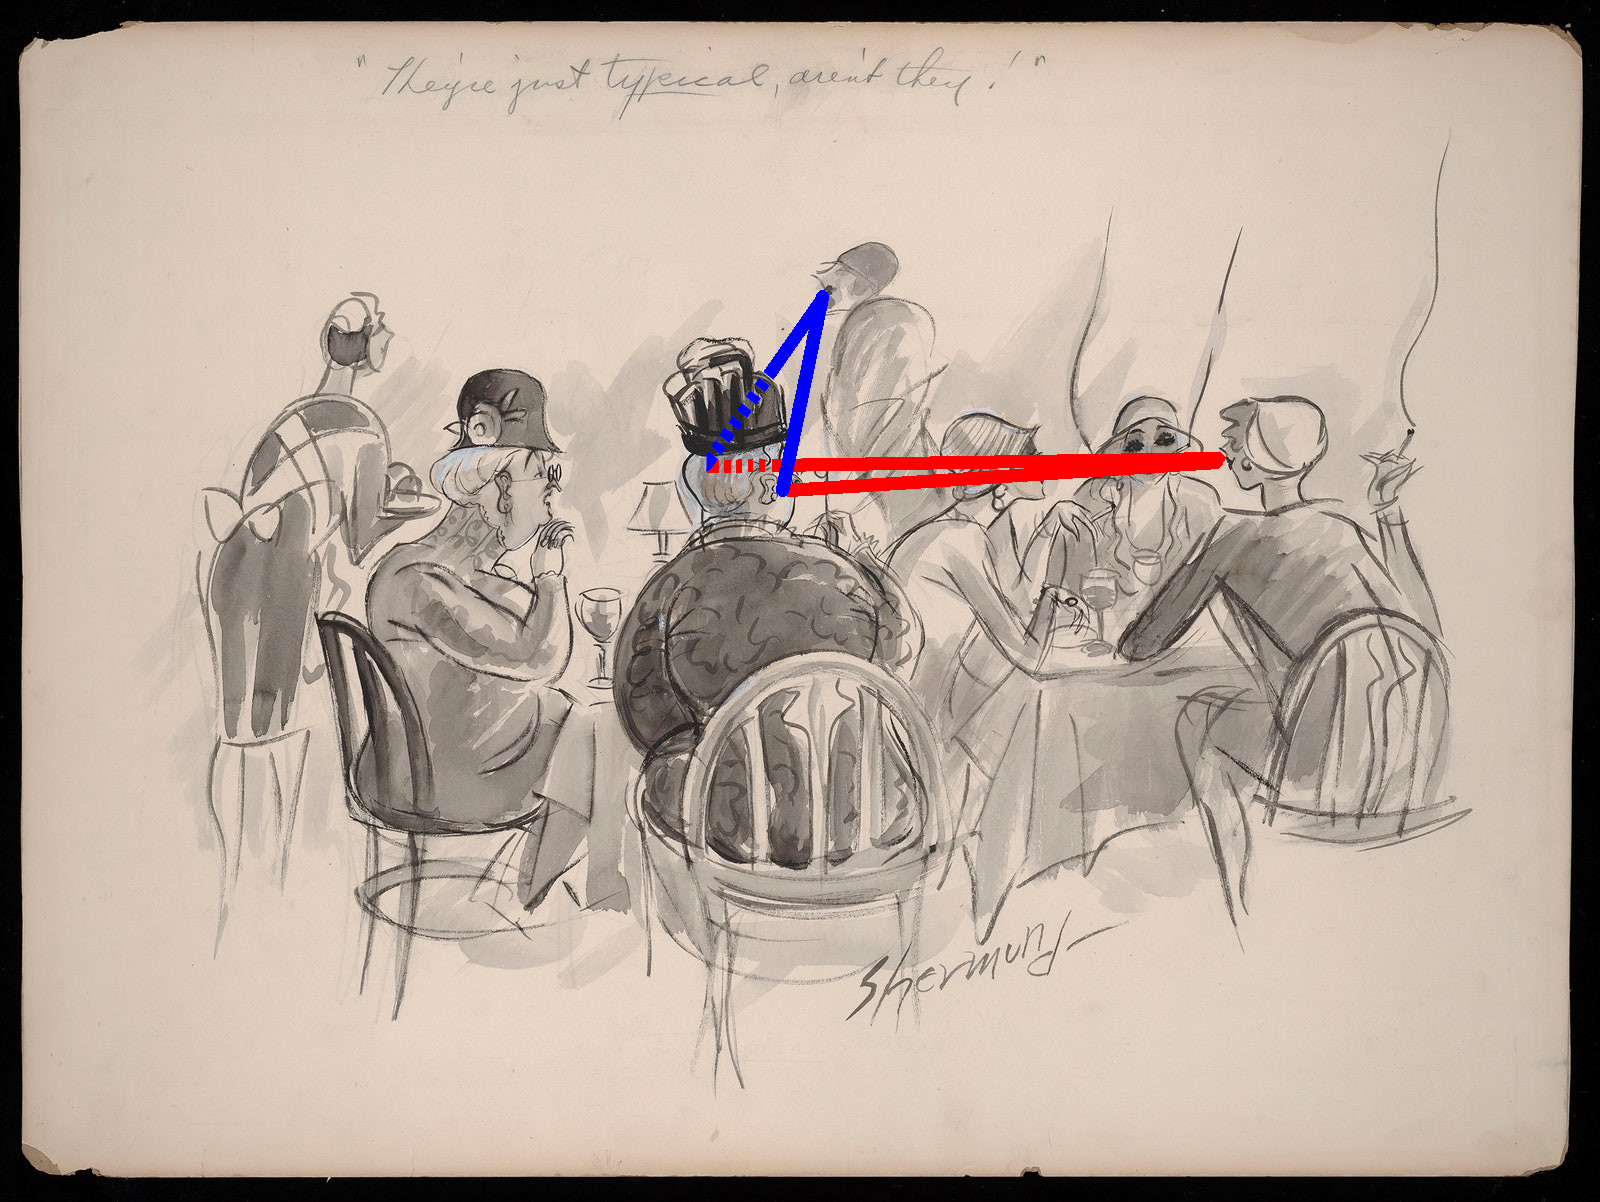
\includegraphics[width=10cm]{Barbara_Shermund_lines.jpg}
  \end{center}
   \vfill
\flushright{\tiny{\cred{}Cartoon by Barbara Shermund.\cbla{}}}
\end{frame}

\begin{frame}{The simple version}
\crish
$$\mathbf{r}(t)=M\mathbf{s}(t)$$
\cbla
with
\begin{itemize}
\item \crish $\mathbf{r}(t)$\cbla{} recordings
\item \crish $\mathbf{s}(t)$\cbla{} sources
\item \crish $M$\cbla{} mixing matrix
\end{itemize}
Assume \crish$$p_{S_1,S_2}(s_1,s_2)=p_{S_1}(s_1)p_{S_2}(s_2)$$\cbla{}
\end{frame}

\begin{frame}{Source separation}
  \crish
$$\mathbf{x}(t)=W\mathbf{r}(t)$$ \cbla{} so that
  \crish$\mathbf{x}(t)$\cbla{} is more-or-less
  \crish$\mathbf{s}(t)$\cbla{} - some rescaling and shuffling may occur.
In this two-to-two example, that means
\crish
$$MW=\mbox{diag}\,(d_1,d_2)$$\cbla{}
or
\crish
$$
MW=\left(\begin{array}{cc}0&d_1\\d_2&0\end{array}\right)
  $$\cbla{}

\end{frame}


\begin{frame}{Source separation}
  \cred
  $$
 \mathbf{ s}\stackrel{\mbox{mixing}}{\longrightarrow}\mathbf{r}=M\mathbf{ s}\stackrel{\mbox{unmixing}}{\longrightarrow}\mathbf{ x}=W\mathbf{r}
 $$
 \cbla
\end{frame}


\begin{frame}{Two approaches}
  \begin{itemize}
  \item \texttt{fastICA}
  \item Infomax
  \end{itemize}
\end{frame}

\begin{frame}{fastICA}

  \texttt{FastICA} maximizes the non-Gau\ss ianity of the components of \crish$\mathbf{x}$\cbla.

  \end{frame}

\end{document}

